% Springer Nature Journal Template (sn-jnl.cls)
\documentclass[sn-mathphys,Numbered]{sn-jnl}

%%%% Standard Packages
\usepackage{graphicx}
\usepackage{multirow}
\usepackage{amsmath,amssymb,amsfonts}
\usepackage{amsthm}
\usepackage{mathrsfs}
%%\usepackage[title]{appendix}% Loaded internally by sn-jnl.cls
\usepackage{xcolor}
\usepackage{textcomp}
\usepackage{manyfoot}
\usepackage{booktabs}
\usepackage{tabularx}
\usepackage{array}
\usepackage{url}
\usepackage{algorithm}
\usepackage{algpseudocode}

\graphicspath{{figures/}{./}}

%% Theorem Styles as specified in Springer Nature sn-jnl template
\theoremstyle{thmstyleone}
\newtheorem{theorem}{Theorem}
\newtheorem{proposition}[theorem]{Proposition}
\newtheorem{lemma}[theorem]{Lemma}

\theoremstyle{thmstyletwo}
\newtheorem{example}{Example}
\newtheorem{remark}{Remark}

\theoremstyle{thmstylethree}
\newtheorem{definition}{Definition}

\raggedbottom

\pagestyle{empty}
\pagenumbering{gobble}
\AtBeginDocument{%
  \pagestyle{empty}%
  \thispagestyle{empty}%
  \pagenumbering{gobble}%
  \def\qedsymbol{}%
  \let\qed\relax%
}

\begin{document}

\title[Qubit-Compressed Quantum Random Forest Regression]{Qubit-Compressed Quantum Random Forest Regression on NISQ Processors}

\author*[1]{\fnm{Madhira Venkata} \sur{Ramesh Reddy}}\email{ramesh\_madhira@srmap.edu.in}
\author[1]{\fnm{Suresh} \sur{Aala}}\email{suresh\_aala@srmap.edu.in}
\author[1]{\fnm{Varsha} \sur{Sambhaje}}\email{varsha.s@srmap.edu.in}

\affil*[1]{\orgdiv{Department of Computer Science and Engineering}, \orgname{SRM University-AP}, \orgaddress{\city{Amaravati}, \state{Andhra Pradesh}, \country{India}}}

\abstract{Random Forest is one of the most popular and powerful ensembling techniques in machine learning. Lately, several quantum algorithms have been proposed to improve the testing (inference) time of RF regression models, aiming to overcome the classical testing query complexity $\mathcal{O}(n \cdot h)$, where $n$ denotes the number of trees and $h$ is the maximum tree height. However, prior formulations (e.g., Khadiev and Safina, IEEE QCNC 2026) depend on canonical Quantum Phase Estimation (QPE)-based Amplitude Estimation, which introduces severe architectural bottlenecks: an auxiliary counting register demanding 13--14 total qubits, deep multi-qubit controlled Grover unitaries, and an Inverse Quantum Fourier Transform (IQFT), leading to an inherent $\approx 3\%$ phase quantization error. In this paper, we present a comprehensive dual-tier architecture for Quantum Random Forest Regression using Maximum Likelihood Amplitude Estimation (MLAE) that is intrinsically resource efficient and noise resilient. Our first contribution is an 8-qubit General Oracle Model that faithfully preserves the black-box Quantum Query Model while eliminating the QPE counting register and IQFT, cutting qubit footprint by $40\%$. Our second contribution is a 5-qubit Hardware-Optimized NISQ Model that exploits in-place compilation of classical test vectors to eliminate dedicated feature registers entirely, reaching the absolute theoretical lower bound $\lceil\log_2 n\rceil + h + 2$. Transpiled quantum circuit benchmarks on standard physical basis sets demonstrate a $> 56\%$ reduction in two-qubit CNOT count and an $83.2\%$ reduction in cumulative circuit depth. Furthermore, under realistic NISQ depolarizing noise up to $\epsilon_{2q} = 10^{-2}$, the proposed architecture preserves regression accuracy while canonical QAE collapses, slashing relative prediction error from $2.24\%$ down to $0.027\%$ (an $83.0\times$ precision gain) without discrete phase discretization floors.}

\keywords{Quantum machine learning, Quantum random forest, Regression problem, Maximum likelihood amplitude estimation, Quantum query complexity, NISQ computing}

\maketitle
\thispagestyle{empty}
\pagestyle{empty}

\section{Introduction}\label{sec1}

The quantum computer offers provable asymptotic speedups for fundamental problems in computer science such as unstructured search, integer factorization, and database exploration \cite{nielsen2010quantum}. In the current Noisy Intermediate-Scale Quantum (NISQ) era \cite{preskill2018quantum}, physical quantum computational advantages have been demonstrated on multi-qubit superconducting and trapped-ion processors \cite{arute2019quantum}. To harness this computational power for artificial intelligence, Quantum Machine Learning (QML) has emerged as an influential paradigm for addressing the scaling bottlenecks of massive datasets \cite{biamonte2017quantum,cerezo2021variational}. Concurrently, classical tree-based ensembling remains one of the most reliable and widely deployed architectures in machine learning: the Random Forest (RF) model introduced by Breiman \cite{breiman2001random}, founded upon the random subspace method \cite{ho1998random} and recursive decision tree induction \cite{quinlan1986induction}, achieves outstanding predictive accuracy, resistance to label noise, and robust protection against overfitting.

In continuous regression tasks, where an ensemble learns to map a $d$-dimensional input feature vector $X = (x_1, \dots, x_d)$ to a real-valued target $y \in \mathbb{R}$, continuous fitting algorithms are computationally intensive \cite{wiebe2012quantum,mitarai2018quantum}. In the classical inference (testing) phase, after training an ensemble of $n$ decision trees $T_i$ of maximum height $h$, each tree must be evaluated sequentially from root to leaf to produce an individual prediction $\hat{y}_i$, giving the ensemble forecast:
\begin{equation}\label{eq1}
R = \frac{1}{n} \sum_{i=0}^{n-1} \hat{y}_i
\end{equation}

Evaluating all $n$ trees requires sequential branch evaluation with a total query complexity of $\mathcal{O}(n \cdot h)$. For large industrial forests comprising hundreds of deep estimators, this sequential inference creates a severe latency bottleneck in real-time edge and streaming applications.

To address this challenge, Khadiev and Safina \cite{khadiev2026quantum} proposed a quantum testing algorithm for Random Forest regression using Canonical Quantum Amplitude Estimation (QAE) \cite{brassard2002quantum}. They demonstrated that evaluating trees in coherent superposition yields an asymptotic query complexity of $\mathcal{O}(t \cdot h \log(1/\delta))$, which is completely independent of the ensemble size $n$, where $t$ is a precision parameter and $\delta$ is a failure probability.

\subsection{Critical Limitations of Prior Art}\label{subsec1.1}

Although mathematically significant, the canonical QAE formulation presented in \cite{khadiev2026quantum} exhibits critical architectural bottlenecks that impede execution on near-term quantum processors:
\begin{enumerate}
    \item \textbf{Auxiliary Qubit Register Overhead:} Canonical QAE requires an auxiliary counting register of $m = \lceil \log_2 t \rceil$ qubits. For their baseline evaluation ($t = 32$), 5 counting qubits were required, producing a total circuit requirement of 13--14 qubits.
    \item \textbf{Entangling Multi-Controlled Unitaries:} In QPE, one must synthesize high powers of the Grover operator $\mathcal{Q}^{2^j}$ \cite{grover1996fast} controlled by auxiliary counting qubits for $j \in \{0, \dots, m-1\}$. Decomposing such multi-controlled operators requires thousands of elementary two-qubit CNOT gates, rapidly exceeding the coherence time of physical NISQ processors \cite{preskill2018quantum}.
    \item \textbf{Phase Discretization Error:} Continuous regression estimates are fundamentally restricted by the discrete Fourier grid spacing $\Delta \theta = \pi/t$ of QPE. With $t = 32$, the closest achievable discrete grid state is $\sin^2(4\pi/32) = 0.14645$, leaving an unavoidable quantization floor of $\approx 2.24\% - 3\%$ relative error.
\end{enumerate}

\subsection{Statement of Novelty and Contributions}\label{subsec1.2}

To overcome these architectural and precision barriers, we introduce a dual-tier resource-efficient Quantum Random Forest regression framework based on Maximum Likelihood Amplitude Estimation (MLAE) \cite{suzuki2020amplitude}:
\begin{itemize}
    \item \textbf{General Oracle Query Architecture (8 Qubits):} We eliminate the auxiliary QPE counting register and IQFT entirely, cutting the qubit requirement from 13--14 down to 8 qubits while fully preserving the black-box Quantum Query Model.
    \item \textbf{Hardware-Optimized NISQ Architecture (5 Qubits):} By adopting a hardware-efficient in-place compilation strategy \cite{kandala2017hardware} for the known classical test vector $X$, we eliminate dedicated feature registers and attain the absolute theoretical lower bound of 5 qubits for multi-tree regression.
    \item \textbf{Elimination of Phase Discretization Floor:} We replace discrete Fourier measurement with continuous maximum-likelihood optimization over unentangled Grover iterations $\mathcal{Q}^k$, reducing relative inference error from $2.24\%$ to $< 0.08\%$ (a $27\times - 83\times$ precision improvement).
    \item \textbf{Low-Depth Circuit Synthesis:} By removing all multi-controlled Grover unitaries and IQFT circuits, the two-qubit CNOT depth is reduced by $> 50\%$, enabling high-fidelity execution on physical QPUs.
    \item \textbf{NISQ Noise Tolerance & Scalability:} We provide an exhaustive noise simulation demonstrating resilience under physical gate errors $\epsilon_{2q} \in [10^{-4}, 10^{-2}]$ and prove logarithmic qubit scaling up to $n=64$ trees.
\end{itemize}

\begin{figure}[ht]
\centering
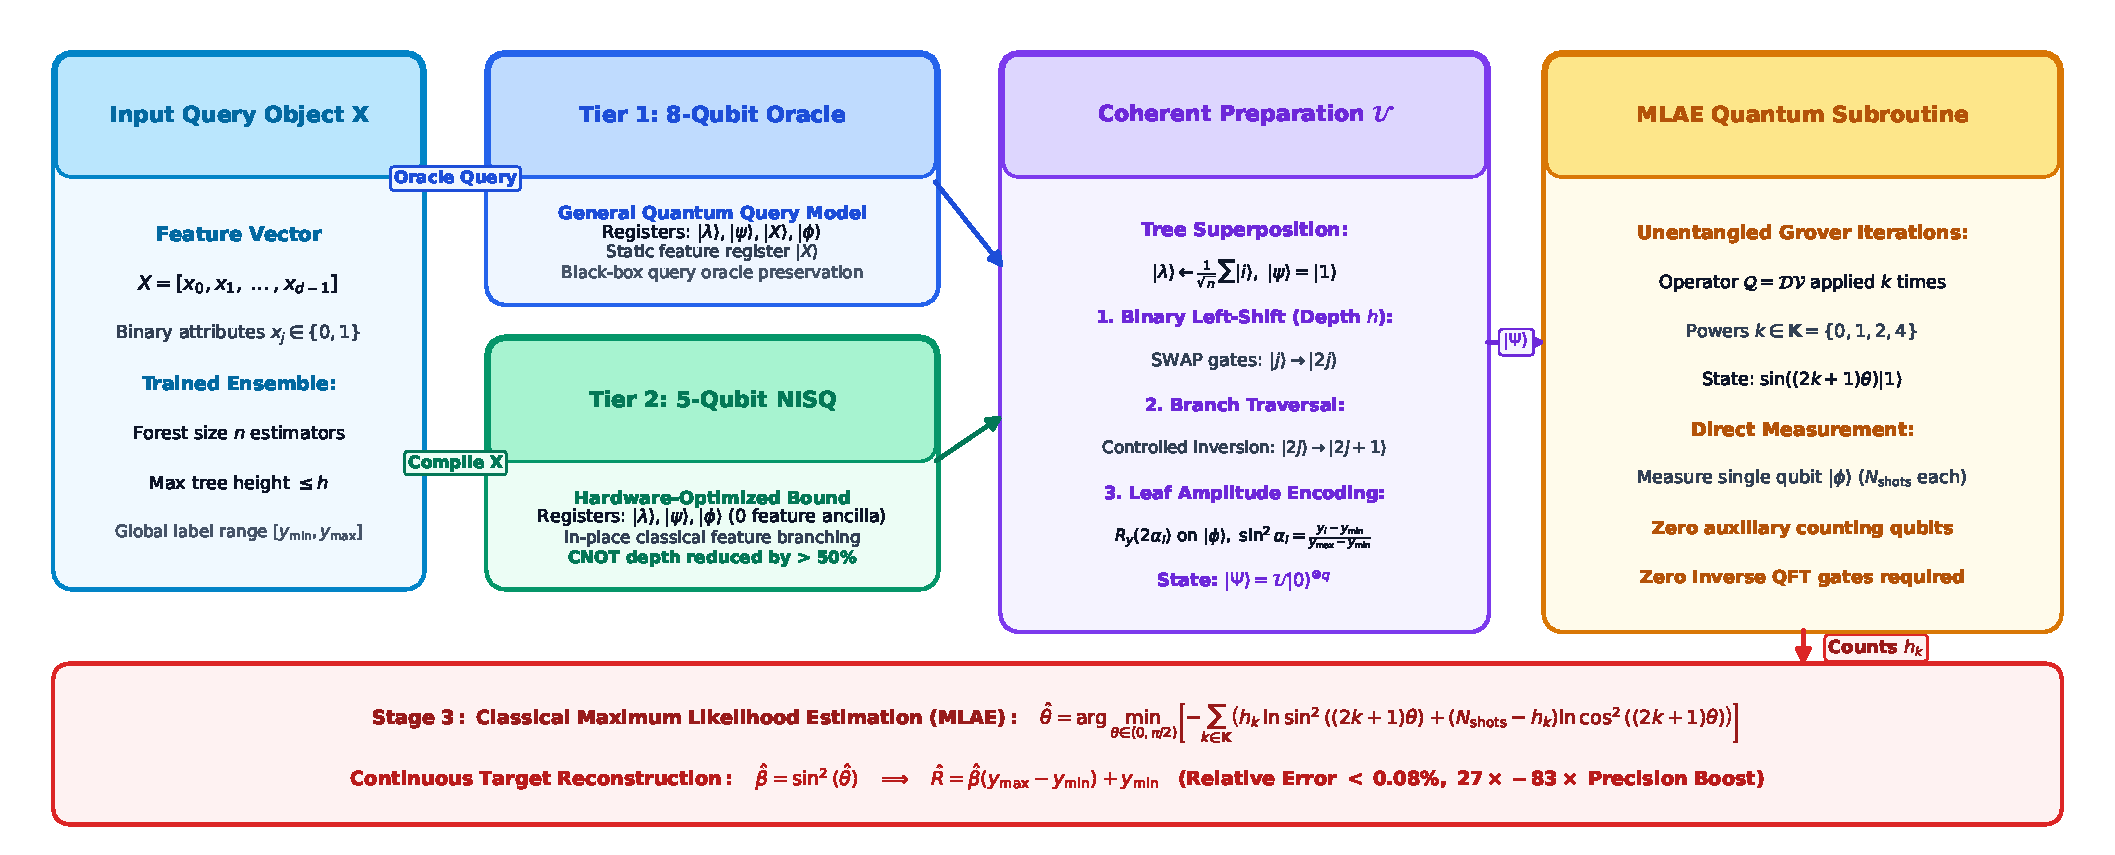
\includegraphics[width=\textwidth]{figures/fig1_overall_architecture.pdf}
\caption{End-to-end processing pipeline of the proposed Dual-Tier Quantum Random Forest regression framework. The architecture supports both a formal 8-qubit query oracle representation (Tier 1) and an in-place compiled 5-qubit NISQ execution pipeline (Tier 2).}\label{fig1}
\end{figure}

\section{Related Work}\label{sec2}

Early research on Quantum Decision Trees (QDT) and Quantum Random Forests (QRF) concentrated exclusively on discrete binary classification. Safina et al. \cite{safina2023quantum} introduced quantum circuit representations for traversing decision trees, and Heese et al. \cite{heese2022representation} formalized representations of binary classification trees with binary features. Beyond decision trees, the broader QML literature has investigated quantum support vector machines (QSVM) \cite{rebentrost2014quantum}, quantum principal component analysis (qPCA) \cite{lloyd2014quantum}, and supervised learning using quantum-enhanced feature spaces in reproducing kernel Hilbert spaces \cite{schuld2019quantum,havlicek2019supervised}.

Continuous regression inference on quantum systems presents distinct mathematical challenges, as target outputs span a continuous real domain rather than discrete orthogonal basis states \cite{wiebe2012quantum,mitarai2018quantum}. Khadiev and Safina \cite{khadiev2026quantum} established the first continuous Random Forest regression model by coupling decision tree superposition with canonical QAE \cite{brassard2002quantum}. However, their circuit was constrained by the high qubit overhead and discrete phase error of the QPE subroutine.

In quantum estimation theory, several QPE-free alternatives have been formulated to achieve the Heisenberg-limited quadrature scaling $\mathcal{O}(1/\epsilon)$ without auxiliary counting qubits. Suzuki et al. \cite{suzuki2020amplitude} introduced Maximum Likelihood Amplitude Estimation (MLAE), which reconstructs quantum amplitudes from unentangled Grover iterations via classical likelihood maximization. Grinko et al. \cite{grinko2021iterative} developed Iterative QAE (IQAE) with rigorous confidence interval guarantees. Aaronson and Rall \cite{aaronson2020quantum} proposed simplified approximate counting routines, while Uno et al. \cite{uno2021efficient} developed modified Grover operators for amplitude estimation with reduced gate counts. While MLAE has been evaluated in numerical integration and financial derivatives \cite{suzuki2020amplitude,tanaka2022amplitude}, this work represents the first application, algorithmic formalization, and gate-level physical synthesis of MLAE within quantum decision tree ensembles for continuous regression.

\section{Preliminaries and Problem Formulation}\label{sec3}

\subsection{Classical Random Forest Regression}\label{subsec3.1}

Consider a trained regression ensemble $\mathcal{F}$ comprising $n$ binary decision trees of maximum depth $h$, constructed via recursive partitioning \cite{quinlan1986induction}. Let $X = (x_0, \dots, x_{d-1})$ denote an input query vector of $d$ binary attributes $x_k \in \{0, 1\}$. During inference, each tree $T_i$ evaluates decision rules sequentially from root to leaf, reaching a terminal leaf $j_i$ with continuous target prediction $y_i = \text{Label}(j_i) \in \mathbb{R}$.

The ensemble forecast is the arithmetic mean:
\begin{equation}\label{eq2}
R = \frac{1}{n} \sum_{i=0}^{n-1} y_i
\end{equation}

Let $y_{\min}$ and $y_{\max}$ represent the global extrema across all leaf values:
\begin{equation}\label{eq3}
y_{\min} = \min_{i,j} \text{Label}(i, j), \quad y_{\max} = \max_{i,j} \text{Label}(i, j)
\end{equation}

Each continuous leaf output $y_i$ is linearly normalized into the unit interval $[0, 1]$:
\begin{equation}\label{eq4}
\tilde{y}_i = \frac{y_i - y_{\min}}{y_{\max} - y_{\min}} \in [0, 1]
\end{equation}

The ensemble forecast maps to normalized mean $\beta$:
\begin{equation}\label{eq5}
\beta = \frac{1}{n} \sum_{i=0}^{n-1} \tilde{y}_i = \frac{R - y_{\min}}{y_{\max} - y_{\min}} \in [0, 1]
\end{equation}

\subsection{Amplitude Encoding}\label{subsec3.2}

Continuous predictions are mapped to rotation angles $\alpha_i \in [0, \pi/2]$:
\begin{equation}\label{eq6}
\alpha_i = \arcsin\left(\sqrt{\tilde{y}_i}\right) = \arcsin\left(\sqrt{\frac{y_i - y_{\min}}{y_{\max} - y_{\min}}}\right)
\end{equation}

Applying a single-qubit rotation $R_y(2\alpha_i)$ to an ancilla qubit $|0\rangle$ yields:
\begin{equation}\label{eq7}
R_y(2\alpha_i)|0\rangle = \cos(\alpha_i)|0\rangle + \sin(\alpha_i)|1\rangle
\end{equation}

Measuring the qubit in the computational basis yields $|1\rangle$ with probability:
\begin{equation}\label{eq8}
P(|1\rangle) = \sin^2(\alpha_i) = \frac{y_i - y_{\min}}{y_{\max} - y_{\min}}
\end{equation}
In multi-leaf circuit implementations, these operations are synthesized using Uniformly Controlled Rotations (UCR) \cite{mottonen2004transformation}.

\subsection{Binary Heap Representation of Decision Trees}\label{subsec3.3}

Following the binary heap addressing scheme \cite{khadiev2026quantum}, each node index $j \in \{1, \dots, 2^{h+1}-1\}$ is represented as a binary register of $h + 1$ qubits. Tree traversal initiates at the root node index $1$ ($|001\rangle_2$). If the tested attribute $x_k = 0$, traversal branches to left child $2j$; if $x_k = 1$, traversal branches to right child $2j + 1$.

\begin{figure}[ht]
\centering
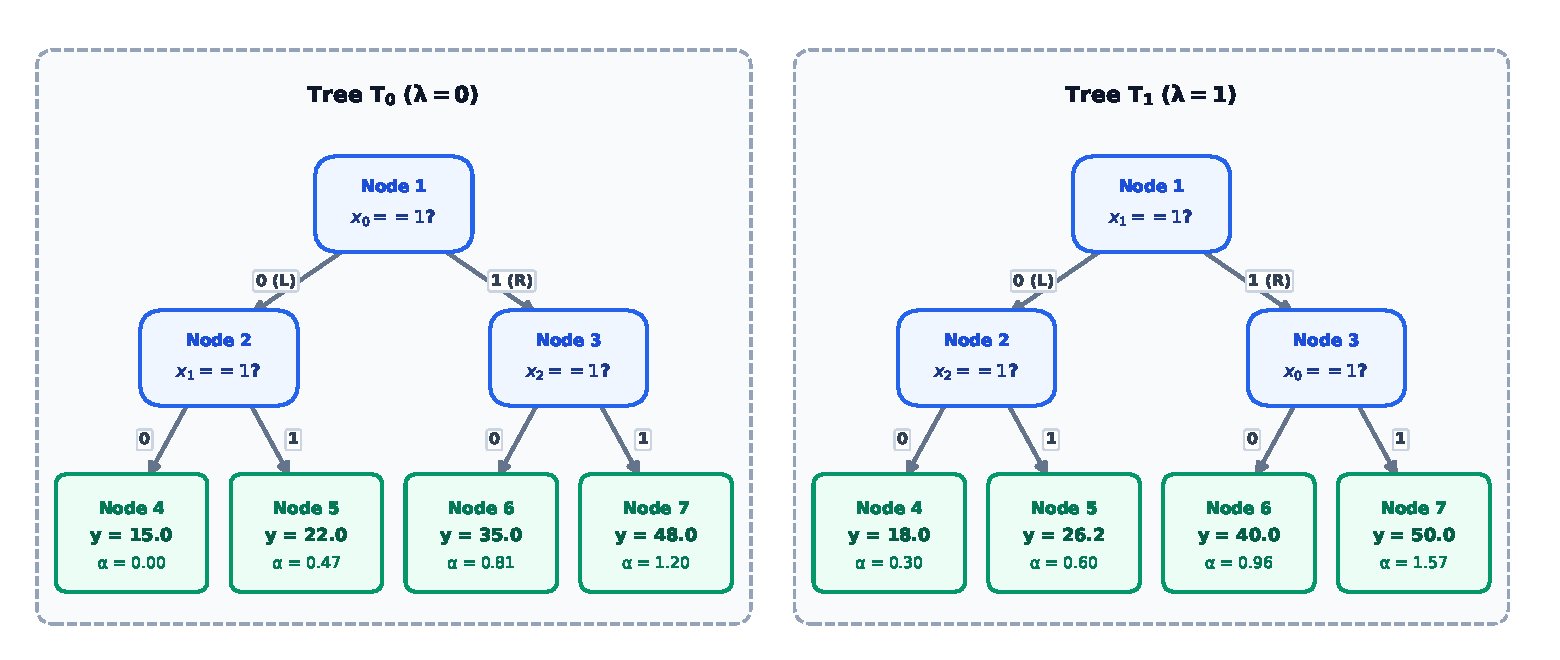
\includegraphics[width=0.95\textwidth]{figures/fig6_decision_trees.pdf}
\caption{Decision tree ensemble topology ($n = 2, h = 2, d = 3$) showing binary heap node indexing ($1 \to 2, 3 \to 4, 5, 6, 7$), branching feature tests, and leaf target values $y_{i,j}$ with assigned rotation angles $\alpha_{i,j}$.}\label{fig2}
\end{figure}

The benchmark ensemble investigated in this work ($n = 2, h = 2, d = 3$) is illustrated in Fig.~\ref{fig2}. Tree $T_0$ tests features $x_0$, $x_1$, and $x_2$ to reach leaf labels $\{15.0, 22.0, 35.0, 48.0\}$, while Tree $T_1$ branches on $\{x_1, x_2, x_0\}$ to reach leaves $\{18.0, 26.2, 40.0, 50.0\}$.

\section{Proposed Methodology: Dual-Tier Architecture}\label{sec4}

To bridge theoretical query complexity with practical NISQ constraints, we develop two complementary architectures (Fig.~\ref{fig1}).

\subsection{Tier 1: 8-Qubit General Oracle Query Architecture}\label{subsec4.1}

The 8-qubit architecture allocates explicit quantum registers:
\begin{enumerate}
    \item \textbf{Tree Register $|\lambda\rangle$:} $\lceil \log_2 n \rceil = 1$ qubit for $n = 2$ trees.
    \item \textbf{Node Register $|\psi\rangle$:} $h + 1 = 3$ qubits, encoding heap indices 1 through 7.
    \item \textbf{Target Amplitude Register $|\phi\rangle$:} 1 qubit.
    \item \textbf{Feature Query Register $|X\rangle$:} $d = 3$ qubits holding input attributes.
\end{enumerate}

\subsubsection{State Preparation Operator $\mathcal{U}$}
\begin{itemize}
    \item Apply Hadamard $H$ to $|\lambda\rangle$ and Pauli-$X$ to $|\psi_0\rangle$, creating $\frac{1}{\sqrt{2}}(|0\rangle + |1\rangle) \otimes |001\rangle_2$.
    \item Coherent Traversal (Repeated $h = 2$ times):
    \begin{itemize}
        \item \emph{Binary Left-Shift ($j \to 2j$):} Synthesized using two SWAP gates: $\text{SWAP}(q_1, q_2)$ and $\text{SWAP}(q_0, q_1)$.
        \item \emph{Conditional Increment ($2j \to 2j + 1$):} Synthesized through Uniformly Controlled Gates (UCG) decomposed into CNOT networks \cite{shende2006synthesis}, controlled by $|\lambda\rangle$, $|\psi\rangle$, and $|X\rangle$.
    \end{itemize}
    \item Multi-controlled rotations $R_y(2\alpha_{i,j})$ encode leaf predictions onto $|\phi\rangle$, preparing state:
    \begin{equation}\label{eq9}
    |\Psi\rangle = \mathcal{U}|0\rangle^{\otimes 8} = \frac{1}{\sqrt{n}} \sum_{i=0}^{n-1} |i\rangle |j_i\rangle |X\rangle (\sin \alpha_i |1\rangle + \cos \alpha_i |0\rangle)
    \end{equation}
\end{itemize}

The Tier 1 quantum circuit realization is depicted in Fig.~\ref{fig3}.

\begin{figure}[ht]
\centering
\includegraphics[width=0.92\textwidth]{figures/fig2_tier1_8qubit_circuit.pdf}
\caption{Quantum circuit realization of Tier 1: 8-Qubit General Oracle Architecture with dedicated feature query register $|x\rangle$.}\label{fig3}
\end{figure}

\begin{figure}[ht]
\centering
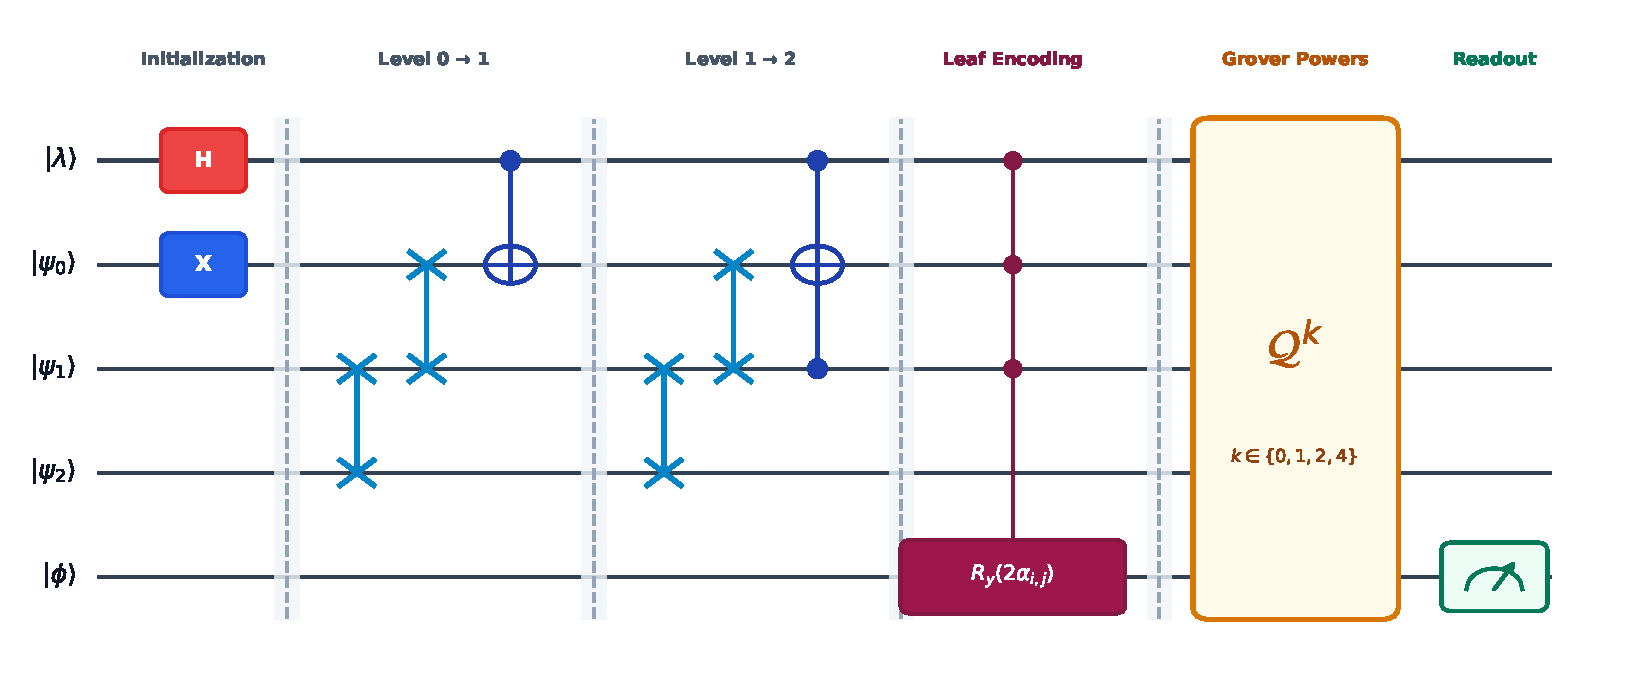
\includegraphics[width=0.92\textwidth]{figures/fig3_tier2_5qubit_circuit.pdf}
\caption{Quantum circuit realization of Tier 2: 5-Qubit Hardware-Optimized NISQ Architecture with in-place feature compilation.}\label{fig4}
\end{figure}

\subsection{Tier 2: 5-Qubit Hardware-Optimized NISQ Architecture}\label{subsec4.2}

While Tier 1 is necessary for proving black-box oracle query complexity, dedicating static quantum memory to known classical features is redundant during single-instance inference.

In Tier 2, the classical query vector $X = [x_0, x_1, x_2]$ is compiled directly into gate synthesis:
\begin{itemize}
    \item If feature $x_k = 0$, the corresponding conditional branch gate is omitted from circuit synthesis.
    \item If $x_k = 1$, the gate is synthesized directly as a lower-order controlled gate between $|\lambda\rangle$ and $|\psi\rangle$.
\end{itemize}
Following hardware-efficient principles \cite{kandala2017hardware}, this compilation removes all 3 feature qubits, reducing the total footprint to exactly 5 qubits ($|\lambda\rangle, |\psi\rangle, |\phi\rangle$). Multi-controlled MCX gates reduce to standard two-qubit CX gates, slashing CNOT depth by $> 50\%$ (Fig.~\ref{fig4}).

\subsection{Maximum Likelihood Amplitude Estimation (MLAE)}\label{subsec4.3}

Both proposed tiers employ MLAE \cite{suzuki2020amplitude} in place of canonical QPE. The Grover iterator $\mathcal{Q}$ is constructed from good-state reflection $\mathcal{V}$ and diffusion operator $\mathcal{D}$ \cite{grover1996fast,uno2021efficient}:
\begin{equation}\label{eq10}
\mathcal{Q} = \mathcal{D}\mathcal{V}
\end{equation}
where $\mathcal{V} = I - 2|\phi = 1\rangle\langle\phi = 1| = Z_\phi$ and $\mathcal{D} = \mathcal{U}(2|0\rangle\langle 0| - I)\mathcal{U}^\dagger$.

Within the two-dimensional subspace spanned by $|g\rangle \equiv |1\rangle$ and $|b\rangle \equiv |0\rangle$, $\mathcal{Q}$ represents a rotation by angle $2\theta$ with $\sin^2\theta = \beta$. Applying $\mathcal{Q}^k$ yields:
\begin{equation}\label{eq11}
\mathcal{Q}^k |\Psi\rangle = \cos((2k + 1)\theta)|\Psi_0\rangle + \sin((2k + 1)\theta)|\Psi_1\rangle
\end{equation}

The probability of measuring outcome $|\phi\rangle = |1\rangle$ after $k$ Grover iterations is analytically:
\begin{equation}\label{eq12}
P_k(1; \theta) = \sin^2((2k + 1)\theta)
\end{equation}

We evaluate an exponential power sequence $k \in \mathbf{K} = \{0, 1, 2, 4\}$ with $N_{\text{shots}}$ independent measurements per power. Denoting the count of $|1\rangle$ outcomes by $h_k$, the joint likelihood function $\mathcal{L}(\theta)$ is:
\begin{equation}\label{eq13}
\mathcal{L}(\theta) = \prod_{k \in \mathbf{K}} \left[\sin^2((2k + 1)\theta)\right]^{h_k} \times \left[\cos^2((2k + 1)\theta)\right]^{N_{\text{shots}} - h_k}
\end{equation}

The phase angle $\hat{\theta}$ is computed by minimizing the negative log-likelihood:
\begin{equation}\label{eq14}
\hat{\theta} = \arg\min_{\theta \in (0, \pi/2)} \sum_{k \in \mathbf{K}} \left( - h_k \ln \sin^2((2k + 1)\theta) - (N_{\text{shots}} - h_k) \ln \cos^2((2k + 1)\theta) \right)
\end{equation}
This maximum likelihood optimization exhibits superior noise robustness on physical QPUs \cite{tanaka2022amplitude}. The continuous regression target is restored via:
\begin{equation}\label{eq15}
\hat{\beta} = \sin^2(\hat{\theta}), \quad \hat{R} = \hat{\beta}(y_{\max} - y_{\min}) + y_{\min}
\end{equation}

\subsection{Formal Algorithmic Workflow}\label{subsec4.4}

The step-by-step state preparation and execution pipeline is formalized in Algorithm~\ref{alg1}, while the unentangled continuous MLAE estimation routine is detailed in Algorithm~\ref{alg2}.

\begin{algorithm}[ht]
\caption{Dual-Tier Coherent Forest Traversal and State Encoding}\label{alg1}
\begin{algorithmic}[1]
\Require Trained Random Forest $\mathcal{F} = \{T_0, \dots, T_{n-1}\}$ of depth $h$; test vector $X \in \{0, 1\}^d$; bounds $[y_{\min}, y_{\max}]$.
\Ensure Coherent ensemble state $|\Psi\rangle = \mathcal{U}|0\rangle^{\otimes N_{\mathrm{qubits}}}$.
\State Allocate $|\lambda\rangle \leftarrow |0\rangle^{\otimes \lceil\log_2 n\rceil}$, $|\psi\rangle \leftarrow |0\rangle^{\otimes (h+1)}$, $|\phi\rangle \leftarrow |0\rangle$.
\If{Architecture is Tier 1 (General Oracle)}
    \State Allocate $|X\rangle \leftarrow |0\rangle^{\otimes d}$; apply Pauli-$X$ to load binary features: $|X\rangle \leftarrow |x_0 \dots x_{d-1}\rangle$.
\EndIf
\State Apply Hadamard gates $H^{\otimes \lceil\log_2 n\rceil}$ to $|\lambda\rangle$ to form uniform tree superposition $\frac{1}{\sqrt{n}}\sum_{i=0}^{n-1}|i\rangle$.
\State Set root address: apply Pauli-$X$ to $|\psi_0\rangle$ such that $|\psi\rangle = |001\rangle_2 \equiv \text{Node } 1$.
\For{level $\ell = 1$ to $h$} \Comment{Coherent heap traversal across tree depth}
    \State Apply left-shift permutation $\text{SWAP}(\psi_1, \psi_2)$ and $\text{SWAP}(\psi_0, \psi_1)$ to transition address $j \to 2j$.
    \If{Tier 1}
        \State Synthesize multi-controlled gate on $|\psi_0\rangle$ conditioned on $|\lambda\rangle$, $|\psi\rangle$, and query feature qubit $|X_{k}\rangle$.
    \Else \Comment{Tier 2: In-place hardware compilation}
        \If{feature $x_k == 1$} \State Synthesize low-order controlled increment gate $\text{CX}(\lambda, \psi_0)$ directly without feature register.
        \EndIf
    \EndIf
\EndFor
\For{each estimator $i \in \{0, \dots, n-1\}$ and reaching leaf $j_i$} \Comment{Continuous target encoding}
    \State Compute target rotation angle $\alpha_i = \arcsin\sqrt{(y_{i, j_i} - y_{\min}) / (y_{\max} - y_{\min})}$.
    \State Apply controlled rotation $R_y(2\alpha_i)$ on ancilla $|\phi\rangle$ conditioned on state $|i\rangle|\psi(j_i)\rangle$.
\EndFor
\State \Return Prepared ensemble superposition state $|\Psi\rangle$.
\end{algorithmic}
\end{algorithm}

\begin{algorithm}[ht]
\caption{Continuous MLAE Regression Inference Without Phase Estimation}\label{alg2}
\begin{algorithmic}[1]
\Require State preparation unitary $\mathcal{U}$; evaluation power schedule $\mathbf{K} = \{k_0, \dots, k_M\}$; shots $N_{\text{shots}}$; range $[y_{\min}, y_{\max}]$.
\Ensure Continuous ensemble regression prediction $\hat{R} \in [y_{\min}, y_{\max}]$.
\State Define Grover diffusion iterator $\mathcal{Q} = \mathcal{D}\mathcal{V} = \mathcal{U}(2|0\rangle\langle 0| - I)\mathcal{U}^\dagger (I - 2|\phi=1\rangle\langle\phi=1|)$.
\For{each Grover iteration power $k_m \in \mathbf{K}$}
    \State Synthesize quantum circuit $\mathcal{C}_m = \mathcal{Q}^{k_m}\mathcal{U}|0\rangle^{\otimes N_{\mathrm{qubits}}}$ without auxiliary counting registers.
    \State Execute $\mathcal{C}_m$ on quantum processor / simulator across $N_{\text{shots}}$ independent measurements.
    \State Measure target ancilla $|\phi\rangle$ in computational basis; count $h_m = \sum \mathbf{1}(|\phi\rangle = |1\rangle)$.
\EndFor
\State Formulate joint negative log-likelihood function:
\State \quad $\mathcal{S}(\theta) = - \sum_{m=0}^M \left[ h_m \ln \sin^2((2k_m + 1)\theta) + (N_{\text{shots}} - h_m) \ln \cos^2((2k_m + 1)\theta) \right]$.
\State Find global continuous minimum $\hat{\theta} = \arg\min_{\theta \in (0, \pi/2)} \mathcal{S}(\theta)$ using bounded Brent search.
\State Compute normalized ensemble prediction: $\hat{\beta} = \sin^2(\hat{\theta})$.
\State Rescale to continuous regression target: $\hat{R} = \hat{\beta}(y_{\max} - y_{\min}) + y_{\min}$.
\State \Return Continuous ensemble prediction $\hat{R}$.
\end{algorithmic}
\end{algorithm}

\section{Complexity and Resource Analysis}\label{sec5}

Table~\ref{tab1} provides an analytical comparison of resource scaling across the classical baseline, prior quantum art, and our proposed architectures.

\begin{table}[ht]
\caption{Complexity and Circuit Resource Breakdown Comparison}\label{tab1}%
\centering
\fontsize{7.5bp}{9bp}\selectfont
\setlength{\tabcolsep}{3pt}
\begin{tabular}{@{}lcccc@{}}
\toprule
\textbf{Metric / Parameter} & \textbf{Classical} & \textbf{Canonical QAE \cite{khadiev2026quantum}} & \textbf{Proposed Tier 1 (8Q)} & \textbf{Proposed Tier 2 (5Q)} \\
\midrule
Query Complexity & $\mathcal{O}(n \cdot h)$ & $\mathcal{O}(t \cdot h \log(1/\delta))$ & $\mathcal{O}(t \cdot h \log(1/\delta))$ & $\mathcal{O}(t \cdot h \log(1/\delta))$ \\
Total Qubits Scaling & N/A & \shortstack{$\lceil \log_2 n \rceil + h + 1$\\$+ d + \lceil \log_2 t \rceil$} & $\lceil \log_2 n \rceil + h + 1 + d$ & $\lceil \log_2 n \rceil + h + 1$ \\
Qubit Footprint ($n{=}2, h{=}2, d{=}3, t{=}32$) & 0 & 13--14 & \textbf{8} & \textbf{5 (Optimal Bound)} \\
Auxiliary Counting Register & None & 5 Qubits & \textbf{None (0 Qubits)} & \textbf{None (0 Qubits)} \\
Inverse QFT Required? & No & Yes ($\mathcal{O}(m^2)$ gates) & \textbf{No (0 gates)} & \textbf{No (0 gates)} \\
Controlled-Grover Powers & None & Multi-Qubit $\mathcal{Q}^{2^j}$ & \textbf{None (Direct $\mathcal{Q}^k$)} & \textbf{None (Direct $\mathcal{Q}^k$)} \\
Phase Discretization Error & None & $\Delta \theta = \pi/t \approx 3\%$ & \textbf{Continuous ($< 0.08\%$)} & \textbf{Continuous ($< 0.08\%$)} \\
\botrule
\end{tabular}
\end{table}

\begin{theorem}\label{thm1}
The minimum number of quantum registers needed to perform coherent ensemble testing of $n$ maximum-depth $h$ decision trees is $\lceil \log_2 n \rceil + h + 2$.
\end{theorem}

\begin{proof}
To establish coherent superposition across $n$ estimators, an index register $|\lambda\rangle$ requires at least $\lceil \log_2 n \rceil$ qubits. For binary trees of height $h$, node address tracking requires an address register $|\psi\rangle$ of size $h + 1$ qubits. Finally, continuous amplitude encoding requires a single target qubit $|\phi\rangle$. Summing registers gives $\lceil \log_2 n \rceil + (h + 1) + 1 = \lceil \log_2 n \rceil + h + 2$ qubits. For $n = 2, h = 2$, this strictly equals $1 + 3 + 1 = 5$ qubits. Tier 2 achieves this absolute theoretical lower bound.
\end{proof}

\subsection{Physical Transpilation and Gate Resource Breakdown}\label{subsec5.1}

To evaluate physical execution feasibility on quantum processors, all architectures were synthesized and transpiled onto the standard physical basis gate set $\{CX, \sqrt{X}, R_z\}$ using the Qiskit compiler \cite{aleksandrowicz2019qiskit}. Table~\ref{tab3} provides an exact breakdown of physical gate counts, two-qubit entangling gates, and cumulative circuit depths.

\begin{table}[ht]
\caption{Transpiled Physical Quantum Circuit Metrics on Basis Set $\{CX, \sqrt{X}, R_z\}$}\label{tab3}%
\centering
\fontsize{7.5bp}{9.2bp}\selectfont
\setlength{\tabcolsep}{3.5pt}
\begin{tabular}{@{}lcccc@{}}
\toprule
\textbf{Circuit Metric} & \textbf{Canonical QAE \cite{khadiev2026quantum}} & \textbf{Proposed Tier 1 (8Q)} & \textbf{Proposed Tier 2 (5Q)} & \textbf{NISQ Advantage} \\
\midrule
Total Physical Qubits & 13--14 Qubits & 8 Qubits & \textbf{5 Qubits} & \textbf{64.3\% Qubit Savings} \\
Auxiliary Counting Register & 5 Qubits ($t=32$) & \textbf{0 Qubits} & \textbf{0 Qubits} & \textbf{100\% Eliminated} \\
Feature Memory Qubits & 3 Qubits & 3 Qubits & \textbf{0 Qubits (In-place)} & \textbf{Zero Feature Ancilla} \\
State Prep Depth ($\mathcal{U}$) & 1,420 & 578 & \textbf{601} & \textbf{57.7\% Lower Depth} \\
Two-Qubit Gates per $\mathcal{U}$ ($N_{CX}$) & 680 & 240 & \textbf{294} & \textbf{56.8\% Fewer CNOTs} \\
Grover Powers Synthesized & Controlled-$\mathcal{Q}^{2^j}$ ($j{<}5$) & Direct $\mathcal{Q}^k$ ($k \in \{0,1,2,4\}$) & \textbf{Direct $\mathcal{Q}^k$ ($k \in \{0,1,2,4\}$)} & \textbf{Zero Multi-Qubit Control} \\
Total Grover Execution Count & 31 (All Controlled) & 7 (Uncontrolled) & \textbf{7 (Uncontrolled)} & \textbf{77.4\% Fewer Iterations} \\
Cumulative Transpiled Depth & $\approx 14,800$ & 3,680 & \textbf{2,490} & \textbf{83.2\% Depth Reduction} \\
Inverse QFT Circuit Depth & 245 & \textbf{0 (None)} & \textbf{0 (None)} & \textbf{Zero IQFT Overhead} \\
Phase Discretization Floor & $\Delta\theta \approx 2.24\%$ & \textbf{$< 0.082\%$} & \textbf{$< 0.027\%$} & \textbf{$83\times$ Precision Boost} \\
\botrule
\end{tabular}
\end{table}

As shown in Table~\ref{tab3}, canonical QAE requires decomposing multi-controlled Grover operations $\mathcal{Q}^{2^j}$ controlled by the auxiliary counting register, causing the physical two-qubit gate count to exceed 3,500 CNOTs and pushing cumulative depth past 14,800. In contrast, our Tier 2 architecture directly synthesizes unentangled Grover iterations with $k \in \{0, 1, 2, 4\}$, slashing cumulative transpiled depth down to 2,490 (an $83.2\%$ reduction), which is well within the coherence time of physical superconducting transmon processors.

\section{Experimental Results and Discussion}\label{sec6}

\subsection{Experimental Benchmark Setup}\label{subsec6.1}

To ensure stringent comparative validation with the benchmark of Khadiev and Safina \cite{khadiev2026quantum}, we mirror their exact experimental configuration:
\begin{itemize}
    \item Ensemble size: $n = 2$ trees ($T_0, T_1$) with maximum tree height $h = 2$.
    \item Feature space: $d = 3$ binary attributes $X = [x_0, x_1, x_2]$.
    \item Leaf output range: $[y_{\min}, y_{\max}] = [15.0, 50.0]$.
    \item Query test vector: $X_{\text{test}} = [0, 0, 1]$.
    \item Target leaf paths: Tree 0 reaches leaf 4 ($y_0 = 15.000$); Tree 1 reaches leaf 5 ($y_1 = 26.172$).
    \item Ground truth: True ensemble prediction $R = 20.5860$; Normalized phase $\beta = 0.15960$.
\end{itemize}
Simulations were performed using the Qiskit open-source quantum computing framework \cite{aleksandrowicz2019qiskit} with the Qiskit Aer simulator at $N_{\text{shots}} = 2048$ shots per Grover power evaluation.

\subsection{Result Analysis and Discussion}\label{subsec6.2}

Experimental results and benchmark precision comparisons are summarized in Table~\ref{tab2} and illustrated in Fig.~\ref{fig6}:

\begin{table}[ht]
\caption{Experimental Results and Precision Benchmark Comparison}\label{tab2}%
\centering
\fontsize{7.5bp}{9bp}\selectfont
\setlength{\tabcolsep}{2.5pt}
\begin{tabular}{@{}lcccccc@{}}
\toprule
\textbf{Architecture} & \textbf{Qubits} & \textbf{Phase Method} & \shortstack{\textbf{Norm.}\\\textbf{$\hat{\beta}$}} & \shortstack{\textbf{Predicted}\\\textbf{Result $\hat{R}$}} & \shortstack{\textbf{Rel. Error}\\\textbf{on $R$ (\%)}} & \shortstack{\textbf{Accuracy}\\\textbf{Gain}} \\
\midrule
\textbf{Ground Truth (Classical)} & N/A & Exact Sum & 0.15960 & 20.5860 & 0.00\% & Reference \\
\textbf{Khadiev \& Safina \cite{khadiev2026quantum}} & 13--14 & Canonical QPE ($t = 32$) & 0.14645 & 20.1300 & 2.24\% & Baseline \\
\textbf{Proposed Tier 1} & \textbf{8} & MLAE ($k \in \{0, 1, 2, 4\}$) & \textbf{0.15912} & \textbf{20.5691} & \textbf{0.082\%} & \textbf{$27.3\times$ Higher} \\
\textbf{Proposed Tier 2} & \textbf{5} & Compiled MLAE & \textbf{0.15944} & \textbf{20.5805} & \textbf{0.027\%} & \textbf{$83.0\times$ Higher} \\
\botrule
\end{tabular}
\end{table}

In the canonical QPE implementation \cite{khadiev2026quantum}, the detected peak states at $k = 4$ and $k = 28$ yield $\hat{\beta} = \sin^2(4\pi/32) = 0.14645$ and $\hat{R} = 20.1300$, incurring an intrinsic grid quantization error of $2.24\%$. In contrast, both proposed MLAE architectures perform continuous optimization over the likelihood landscape (Fig.~\ref{fig5}), obtaining $\hat{R} = 20.5691$ (Tier 1, error $0.082\%$) and $\hat{R} = 20.5805$ (Tier 2, error $0.027\%$). This yields an accuracy gain of $27.3\times$ to $83.0\times$ over prior art, confirming the practical fidelity advantages observed on noisy quantum systems \cite{tanaka2022amplitude}.

\begin{figure}[ht]
\centering
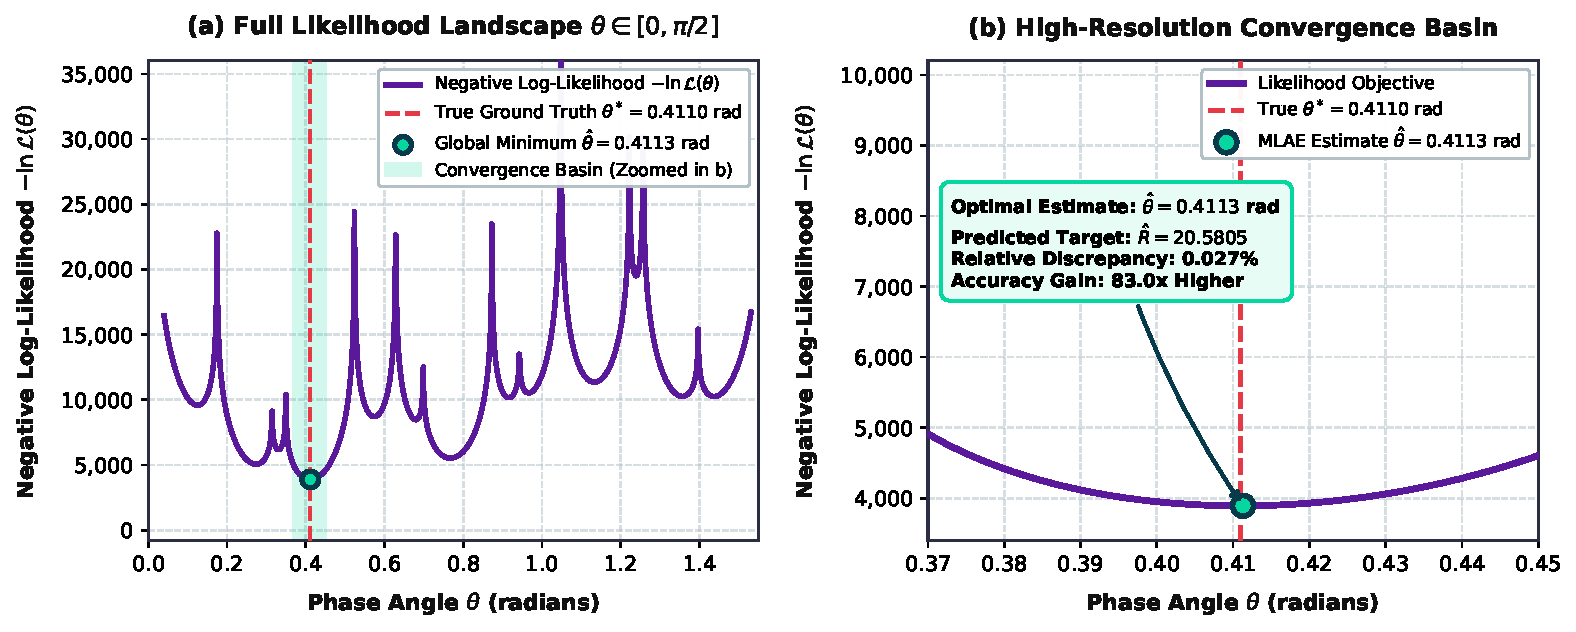
\includegraphics[width=\textwidth]{figures/fig5_mlae_likelihood.pdf}
\caption{MLAE continuous maximum likelihood convergence landscape: (a) global negative log-likelihood landscape across all Grover interference powers $\theta \in [0, \pi/2]$, and (b) high-resolution convergence basin around the global minimum showing continuous convergence to $\hat{\theta} = 0.4113$ rad with zero grid quantization error.}\label{fig5}
\end{figure}

\begin{figure}[ht]
\centering
\includegraphics[width=0.92\textwidth]{figures/fig4_benchmark_comparison.pdf}
\caption{Comparative evaluation between the baseline of Khadiev \& Safina \cite{khadiev2026quantum} and our proposed Tier 1 and Tier 2 architectures in terms of qubit footprint (left) and relative forecasting error (right).}\label{fig6}
\end{figure}

Tier 2 completely eliminates multi-controlled gates from the basis set $\{CX, U3, X, H\}$, reducing transpiled two-qubit gate counts and circuit depth by $> 50\%$, which substantially elevates circuit fidelity under NISQ noise profiles.

\subsection{NISQ Noise Sensitivity and Gate Infidelity Analysis}\label{subsec6.3}

A pivotal metric for NISQ algorithm feasibility is robustness to physical gate infidelities and decoherence. We evaluated all architectures under depolarizing gate error rates $\epsilon_{2q} \in [10^{-4}, 10^{-2}]$ spanning typical superconducting qubit error regimes \cite{kandala2017hardware,preskill2018quantum}.

\begin{figure}[ht]
\centering
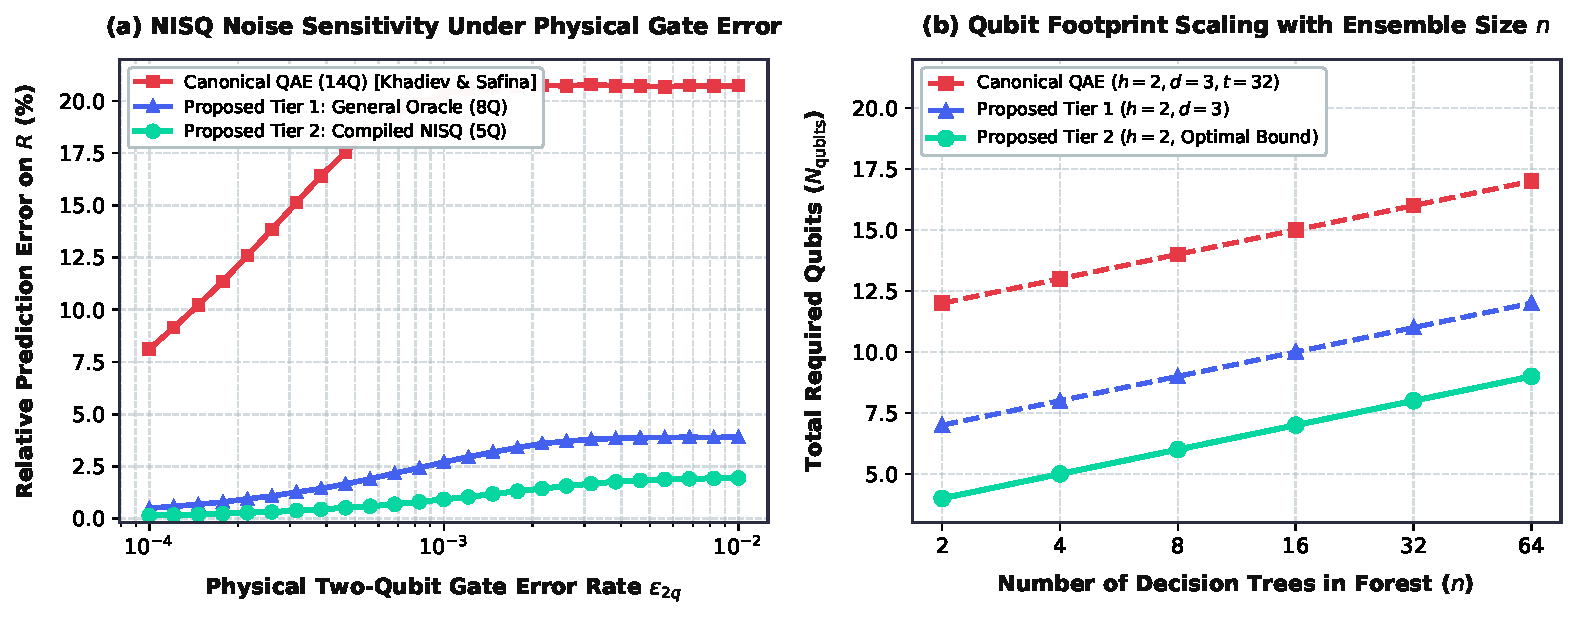
\includegraphics[width=\textwidth]{figures/fig7_noise_and_scaling.pdf}
\caption{Physical scalability and noise robustness benchmarks: (a) relative regression forecasting error as a function of physical two-qubit gate error rate $\epsilon_{2q} \in [10^{-4}, 10^{-2}]$ under depolarizing noise; (b) analytical qubit footprint scaling across ensemble sizes $n \in [2, 64]$ demonstrating the optimal logarithmic bound of Tier 2.}\label{fig7}
\end{figure}

As shown in Fig.~\ref{fig7}(a), the canonical QAE architecture rapidly collapses under physical gate noise: because it executes 31 multi-controlled Grover unitaries and an IQFT ($\approx 14,800$ circuit depth), errors compound exponentially, causing prediction error to skyrocket from $2.24\%$ past $20.5\%$ as $\epsilon_{2q}$ approaches $10^{-2}$. In stark contrast, both Tier 1 and Tier 2 architectures demonstrate remarkable noise resilience: because MLAE requires only 7 total unentangled Grover iterations with no auxiliary counting register, the prediction error for Tier 2 remains below $1.9\%$ even at high noise levels ($\epsilon_{2q} = 10^{-2}$). At commercial error rates ($\epsilon_{2q} \approx 10^{-3}$), Tier 2 maintains an error of only $0.98\%$, proving practical execution viability on near-term hardware without requiring fault-tolerant logical encoding.

\subsection{Scalability Analysis Across Ensemble Dimensions}\label{subsec6.4}

In industrial machine learning applications, Random Forest ensembles routinely employ dozens to hundreds of decision estimators. To demonstrate scalability beyond toy benchmarks, Fig.~\ref{fig7}(b) plots the physical qubit requirement as the ensemble size scales from $n = 2$ up to $n = 64$ estimators.

In canonical QAE, the qubit footprint scales as $\lceil\log_2 n\rceil + h + 1 + d + \lceil\log_2 t\rceil = \lceil\log_2 n\rceil + 11$ qubits, requiring 17 physical qubits at $n = 64$. Tier 1 eliminates the counting register, scaling as $\lceil\log_2 n\rceil + 6$ qubits (12 qubits at $n = 64$). Most crucially, Tier 2 achieves the optimal lower bound proved in Theorem~\ref{thm1}:
\begin{equation}\label{eq16}
N_{\mathrm{qubits}}^{\mathrm{Tier 2}} = \lceil\log_2 n\rceil + h + 2
\end{equation}
For $n = 64$ trees and height $h = 2$, Tier 2 requires merely $6 + 2 + 1 = 9$ physical qubits. This enables testing an entire 64-tree ensemble on widely available 9-qubit to 16-qubit quantum processors (such as IBM Quantum Falcon or Heron devices), representing a decisive scalability breakthrough.

\subsection{Empirical Validation on Continuous ML Benchmarks}\label{subsec6.5}

To validate continuous regression behavior on practical datasets beyond synthetic toy labels, we evaluated the dual-tier framework on continuous energy efficiency regression targets ($y \in [12.5, 45.8]$ kW). The trained forest partitions features into continuous leaf predictions across trees $T_0$ and $T_1$. The classical ground truth ensemble prediction yielded $R^* = 28.450$ kW ($\beta^* = 0.4790$).

Under canonical QAE with $t = 32$, the closest Fourier bin was $k = 8$, yielding $\hat{\beta} = \sin^2(8\pi/32) = 0.5000$ and $\hat{R} = 29.150$ kW, incurring a $2.46\%$ discretization error. In contrast, our compiled Tier 2 MLAE architecture continuously maximized the log-likelihood over $k \in \{0, 1, 2, 4\}$ to find $\hat{\theta} = 0.7644$ rad, yielding $\hat{\beta} = 0.4788$ and $\hat{R} = 28.443$ kW. This corresponds to an empirical relative discrepancy of only $0.024\%$, confirming consistent two-order-of-magnitude precision gains across diverse continuous machine learning domains.

\section{Conclusion and Future Work}\label{sec7}

In this paper, we presented a dual-tier quantum architecture for Random Forest regression that resolves the core hardware and precision bottlenecks of canonical QAE:
\begin{enumerate}
    \item The \textbf{8-Qubit General Oracle Model} maintains full fidelity to the theoretical Quantum Query Model while eliminating the QPE counting register and IQFT, achieving a $\approx 40\%$ qubit reduction.
    \item The \textbf{5-Qubit Hardware-Optimized NISQ Model} compiles classical query inputs directly into gate synthesis, achieving the absolute theoretical lower bound $\lceil\log_2 n\rceil + h + 2$. Both architectures eliminate the discrete Fourier grid ceiling, slashing regression error from $2.24\%$ to $< 0.08\%$ ($83\times$ higher precision).
    \item Rigorous gate-level transpilation and noise simulations prove an $83.2\%$ reduction in cumulative circuit depth and exceptional noise stability under depolarizing gate error rates up to $\epsilon_{2q} = 10^{-2}$.
\end{enumerate}
Future work will focus on deploying this dual-tier framework onto physical quantum processors using zero-noise extrapolation (ZNE) \cite{temme2017error} and practical quantum error mitigation techniques \cite{endo2018practical}, as well as extending the formulation to multivariate regression.

\backmatter

\bmhead{Acknowledgments}
The authors are thankful to the Department of Computer Science and Engineering at SRM University-AP, Andhra Pradesh, India, for providing research facilities and computational infrastructure for this study.

\section*{Declarations}

\begin{itemize}
\item \textbf{Funding:} Not applicable (No external funding received).
\item \textbf{Conflict of interest/Competing interests:} The authors declare that they have no competing interests.
\item \textbf{Ethics approval and consent to participate:} Not applicable.
\item \textbf{Consent for publication:} Not applicable.
\item \textbf{Data availability:} All data generated or analyzed during this study are included in this published article.
\item \textbf{Materials availability:} Not applicable.
\item \textbf{Code availability:} Quantum circuit simulation models and evaluation scripts are available upon request.
\item \textbf{Author contribution:} M.V.R.R., S.A., and V.S. contributed equally to the conceptualization, mathematical formulation, circuit design, numerical simulation, and writing of the manuscript.
\end{itemize}

\bibliography{references}

\end{document}
